\chapter{Модель Поттса с числом состояний спина \texorpdfstring{$q=3$}{q=3} на решетке Кагоме}

\section{Ведение}

Нами приводятся результаты исследования трехвершинной модели Поттса на решетке Кагоме методом Ванга-Ландау \cite{mma-bib-1, mma-bib-2}. Модель Поттса была предложена в 1952 году Поттсом по предложению С. Домба. Модель задается числом состояний $q$, в которых может находиться спин на произвольной решетке.

Гамильтониан модели Поттса с числом состояний $q=3$ на решетке Кагоме может быть представлен в следующем виде:
\begin{equation}
    \label{mma-eq-1}
    H = - J_1 \sum_{i, j} \cos \theta_{i, j} - J_2 \sum_{i, k} \cos \theta_{i, k},
\end{equation}
где $J_1$ и $J_2$ -- параметры обменного взаимодействия для ближайших и вторых ближайших соседей. $\theta_{i,j}$, $\theta_{i,k}$ -- углы между взаимодействующими спинами $S_i - S_j$ и $S_i - S_k$ соответственно. Отметим, что в данной работе рассматривается случай ферромагнитного обменного взаимодействия между ближайшими соседями ($J_1 = 1$) и конкурирующего антиферромагнитного взаимодействия между следующими за ближайшими соседями ($J_2 \leq 0$).

Схематическое и цветовое представление модели представлено на рисунке \ref{mma-fig-1}. На вставке приведены направления спинов для каждого из 3 значений спина и соответствующее цветовое представление. Также представлены взаимодействия между первыми и вторыми ближайшими соседями (каждый спин имеет 4 ближайших и 4 следующих за ближайшими соседа).
\begin{figure}[h]
    \begin{center}
        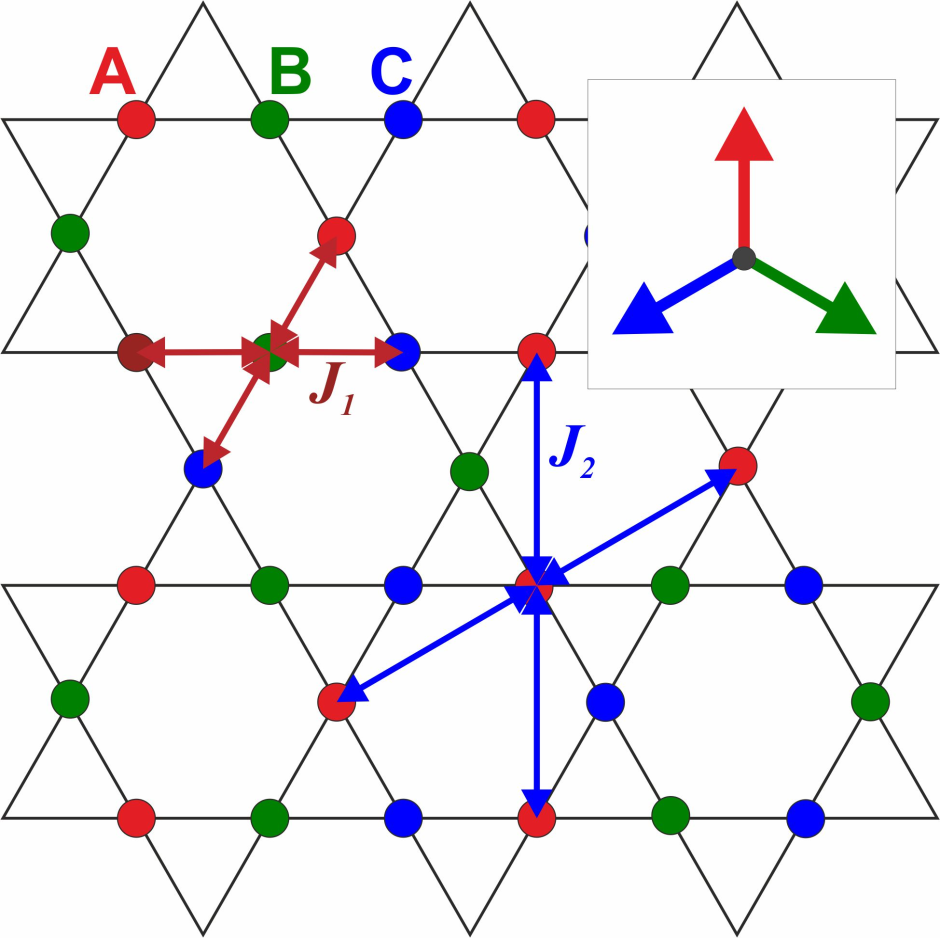
\includegraphics[width=0.4\textwidth]{mma/image2.png}
    \end{center}
    \caption{Модель Поттса с числом состояний спина $q = 3$ на решетке Кагоме.}
    \label{mma-fig-1}
\end{figure}

В данной работе значения обменных интегралов нами были приняты равными: $J_1 = 1$, а $J_2$ было принято антиферромагнитным и менялось по величине от 0 до 2. Таким образом, в исследованной нами в данной работе модели Поттса на решетке Кагоме учитывается ферромагнитное взаимодействие между ближайшими соседями спина и антиферромагнитное взаимодействие разной величины между следующими за ближайшими соседями. Для учета влияния размеров системы на термодинамические свойства исследовались системы с линейными размерами $L=12$ и $L=36$.


\section{Метод исследований}

Исследования проводились на основе алгоритма Ванга-Ландау метода Монте-Карло (МК) \cite{mma-bib-10, mma-bib-11, mma-bib-12, mma-bib-13, mma-bib-14, mma-bib-15}. Данный алгоритм является реализацией метода энтропийного моделирования и его основной особенностью является возможность расчета функции плотности состояний системы, зная которую можно легко вычислить любые интересующие нас термодинамические параметры системы.

Алгоритм Ванга-Ландау является разновидностью энтропийного моделирования и, как показывает опыт его применения в последние годы, является весьма эффективным для исследования различных дискретных спиновых систем \cite{mma-bib-14}.

Алгоритм Ванга-Ландау основан на том, что совершая случайное блуждание в пространстве энергий с вероятностями, обратно пропорциональными плотности состояний $g(E)$, мы получаем равномерное распределение по энергиям. Подобрав вероятности перехода такими, что посещение всех энергетических состояний стало бы равномерным, можно получить изначально неизвестную плотность состояний $g(E)$, зная которую можно вычислить значения необходимых термодинамических параметров при любой температуре. Так как плотность состояний $g(E)$ очень быстро растет с увеличением размеров исследуемых систем, для удобства хранения и обработки больших чисел пользуются величиной $\ln g(E)$.

Важным обстоятельством является то, что плотность состояний $g(E)$ не зависит от температуры, следовательно, рассчитав ее однократно, мы можем вычислить значения любых термодинамических параметров системы при любой ненулевой температуре.

В данной работе нами алгоритм Ванга-Ландау был использован в следующем виде \cite{mma-bib-10, mma-bib-11, mma-bib-12}:
\begin{itemize}
    \item Задается произвольная начальная конфигурация спинов. Стартовые значения плотности состояний $g(E) = 1$, гистограммы распределений по энергиям $H(E) = 0$ и начальное значение модификационного фактора $f = f_0 = e^1 \approx 2.71828$.
    \item Многократно совершаем шаги в фазовом пространстве, пока не получим относительно плоскую гистограмму $H(E)$ (т.е. пока не будут посещены примерно одинаковое количество раз все возможные энергетические состояния системы). В качестве критерия <<плоскости>> гистограммы нами принималось условие отклонения числа посещений всех возможных (с ненулевой плотностью $g(E) \neq 1$) энергетических состояний на величину не более чем на 10\% от среднего значения по системе.
    \item При этом вероятность перехода из состояния с энергией $E_1$ в состояние с энергией $E_2$ определяется по формуле $p = g(E_1)/g(E_2)$. Если переход в состояние с энергией $E_2$ состоялся, то для энергии $E_2$ проводится модификация плотности состояния $g(E_2) \to f \times g(E_2)$, и гистограммы $H(E_2) \to H(E_2) + 1$ иначе меняем параметры для энергии $E_1$ $g(E_1) \to f \times g(E_1)$, $H(E_1) \to H(E_1) + 1$.
    \item Если гистограмма стала <<плоской>> то: обнуляем гистограмму $H(E) \to 0$,  уменьшаем модификационный фактор $f \to \sqrt{f}$, и продолжаем снова и снова, пока модификационный фактор $f \geq f_{\min}$. В качестве минимального значения модификационного фактора нами принималось $f_{\min} = 1.0000000001$.
    \item Каждый раз при достижении энергетического минимума нами проводился анализ магнитной структуры основного состояния и его запись в графический файл. При этом проводилось сравнение полученной конфигурации с ранее полученными и только при обнаружении новой уникальной конфигурации производится ее сохранение в графический файл. Далее данная структура заносится в специальную базу данных для данной модели для дальнейшего сравнения. Данная процедура позволяет избежать дублирования в графических файлах многократно встречающихся состояний с одинаковой магнитной структурой.
    \item После расчета плотности состояний системы для любой интересующей нас температуры рассчитываются различные термодинамические параметры, такие как, энтропия, внутренняя энергия, свободная энергия, теплоемкость, намагниченность, восприимчивость и т.д. Некоторые формулы (\eqref{mma-eq-2}, \eqref{mma-eq-3}, \eqref{mma-eq-4}, \eqref{mma-eq-5}, \eqref{mma-eq-6}), для расчета термодинамических параметров приведены ниже.
    Более подробно алгоритм Ванга-Ландау изложен в работах \cite{mma-bib-10, mma-bib-11, mma-bib-12, mma-bib-13, mma-bib-14, mma-bib-15}.
\end{itemize}

\section{Результаты исследований}

На рисунке \ref{mma-fig-2} приведены значения энергии основного состояния системы при различных значениях взаимодействий $J_1$ и $J_2$. Как видно из графика, в данной модели при низких температурах возможно ферромагнитное упорядочение (FM) (при $J_2 > -0.5$), триплетное антиферромагнитное упорядочение (TAFM) (при $J_2 < -0.5$) или возникновение неупорядоченного фрустрированного состояния ($J_2 = -0.5$).
\begin{figure}[h]
    \begin{center}
        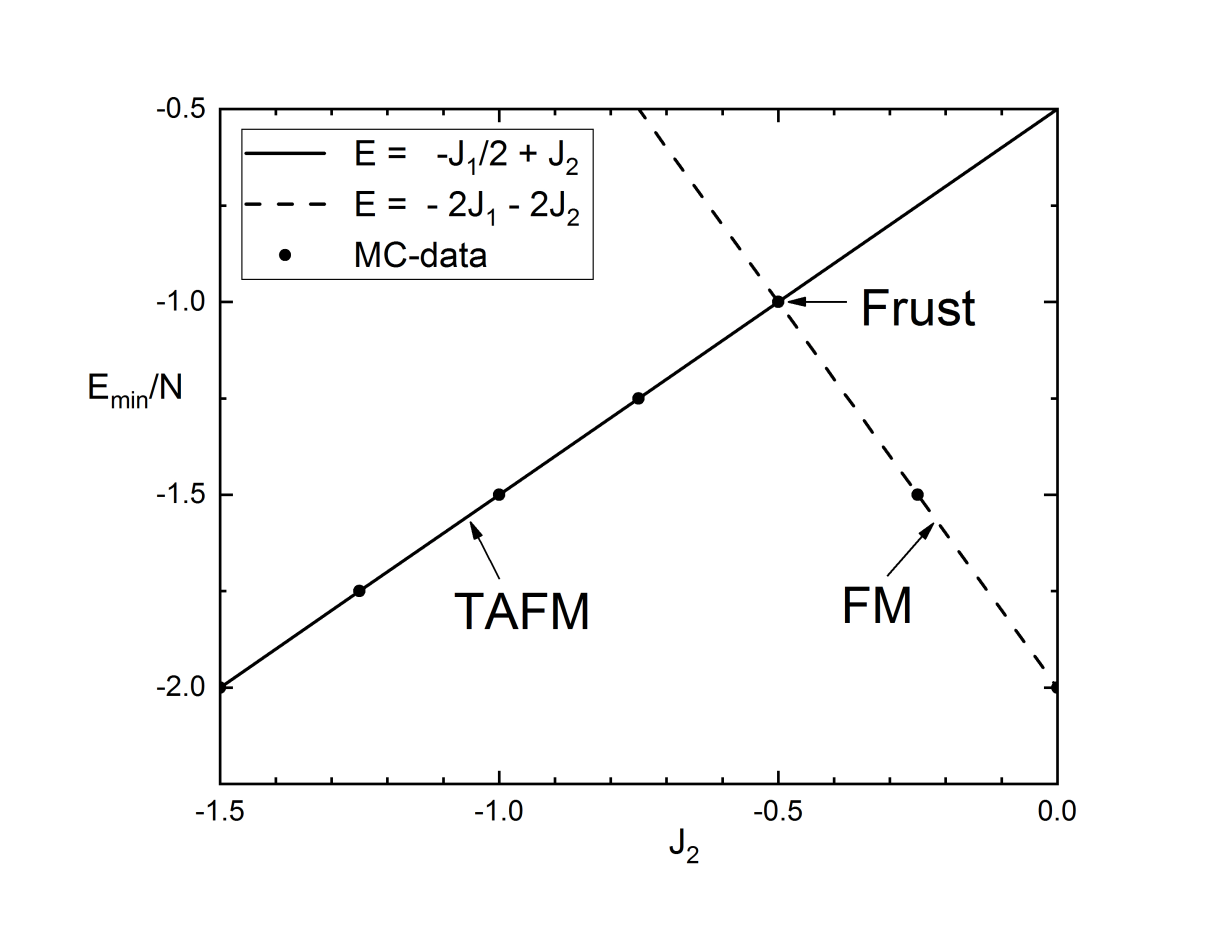
\includegraphics[width=0.5\textwidth]{mma/image19.png}
    \end{center}
    \caption{Энергия основного состояния системы.}
    \label{mma-fig-2}
\end{figure}

Плотность состояний системы $g(E)$ при различных значениях обменных взаимодействий $J_1$ и $J_2$ для систем с линейными размерами $L = 12$ и $L = 36$ приведены на рисунке \ref{mma-fig-3}. На графике приведены плотности состояний для всех трех областей, приведенных на рисунке \ref{mma-fig-2}. Как видно из рисунка, основное состояние системы при $J_2 = -0.5$ сильно вырождено, что обусловлено наличием в данном случае фрустрации в системе, а в остальных случаях вырождение не наблюдается.
\begin{figure}[h]
    \begin{center}
        \begin{subfigure}{0.45\textwidth}
            \begin{center}
                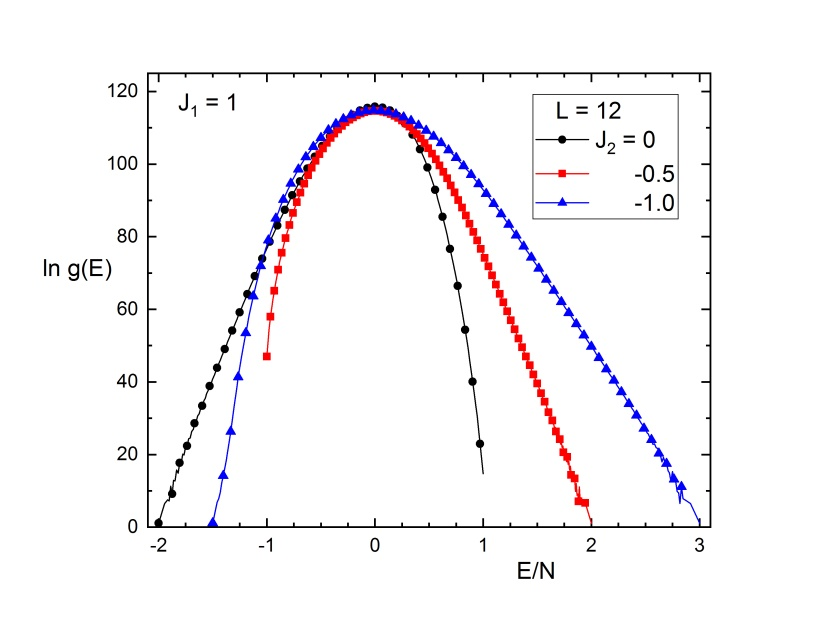
\includegraphics[width=1.0\textwidth]{mma/image20.jpeg}
            \end{center}
        \end{subfigure}
        \begin{subfigure}{0.45\textwidth}
            \begin{center}
                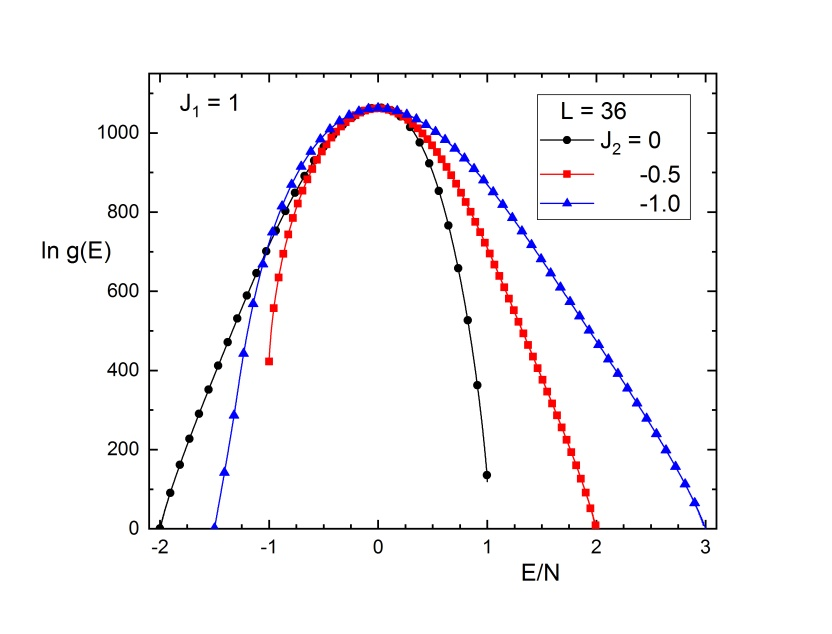
\includegraphics[width=1.0\textwidth]{mma/image21.jpeg}
            \end{center}
        \end{subfigure}
    \end{center}
    \caption{Плотность состояний $g(E)$ для трехвершинной модели Поттса на решетке Кагоме при различных значениях обменных взаимодействий $J_1$ и $J_2$.}
    \label{mma-fig-3}
\end{figure}

На рисунках \ref{mma-fig-4}, \ref{mma-fig-5}, \ref{mma-fig-6} приведены структуры основного состояния для ферромагнитной области ($J_2 > -0.5$), области фрустраций ($J_2 = -0.5$) и триплетной антиферромагнитной области ($J_2 < -0.5$).
\begin{figure}[h]
    \begin{center}
        \begin{subfigure}{0.3\textwidth}
            \begin{center}
                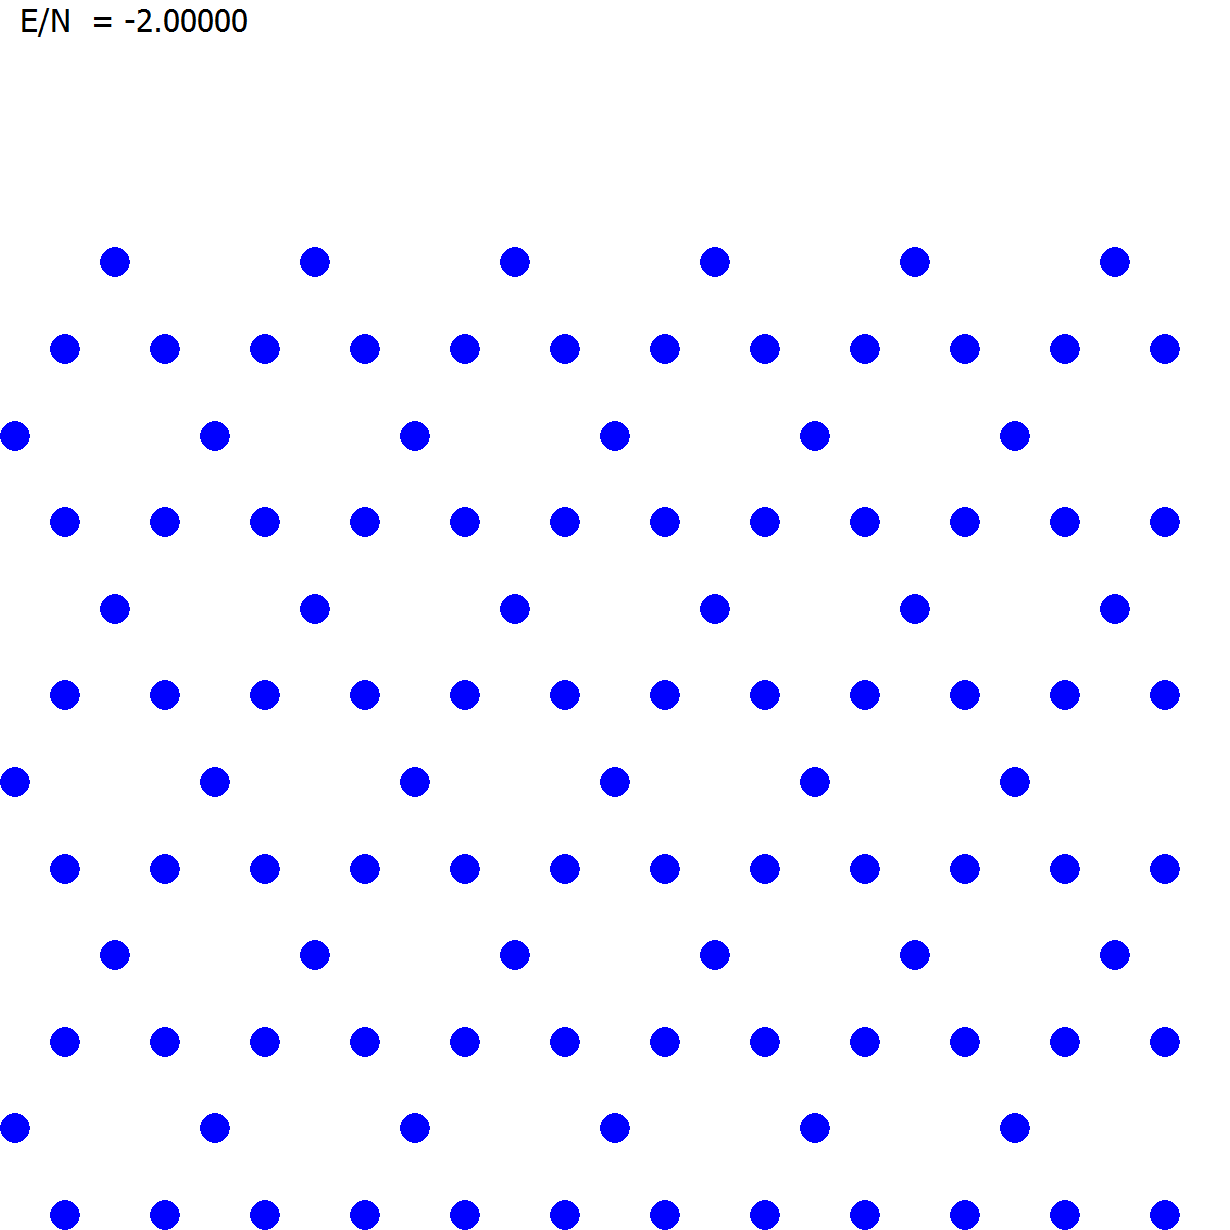
\includegraphics[width=1.0\textwidth]{mma/image24.png}
            \end{center}
            \caption{$J_2 > -0.5$.}
            \label{mma-fig-4}
        \end{subfigure}
        \begin{subfigure}{0.3\textwidth}
            \begin{center}
                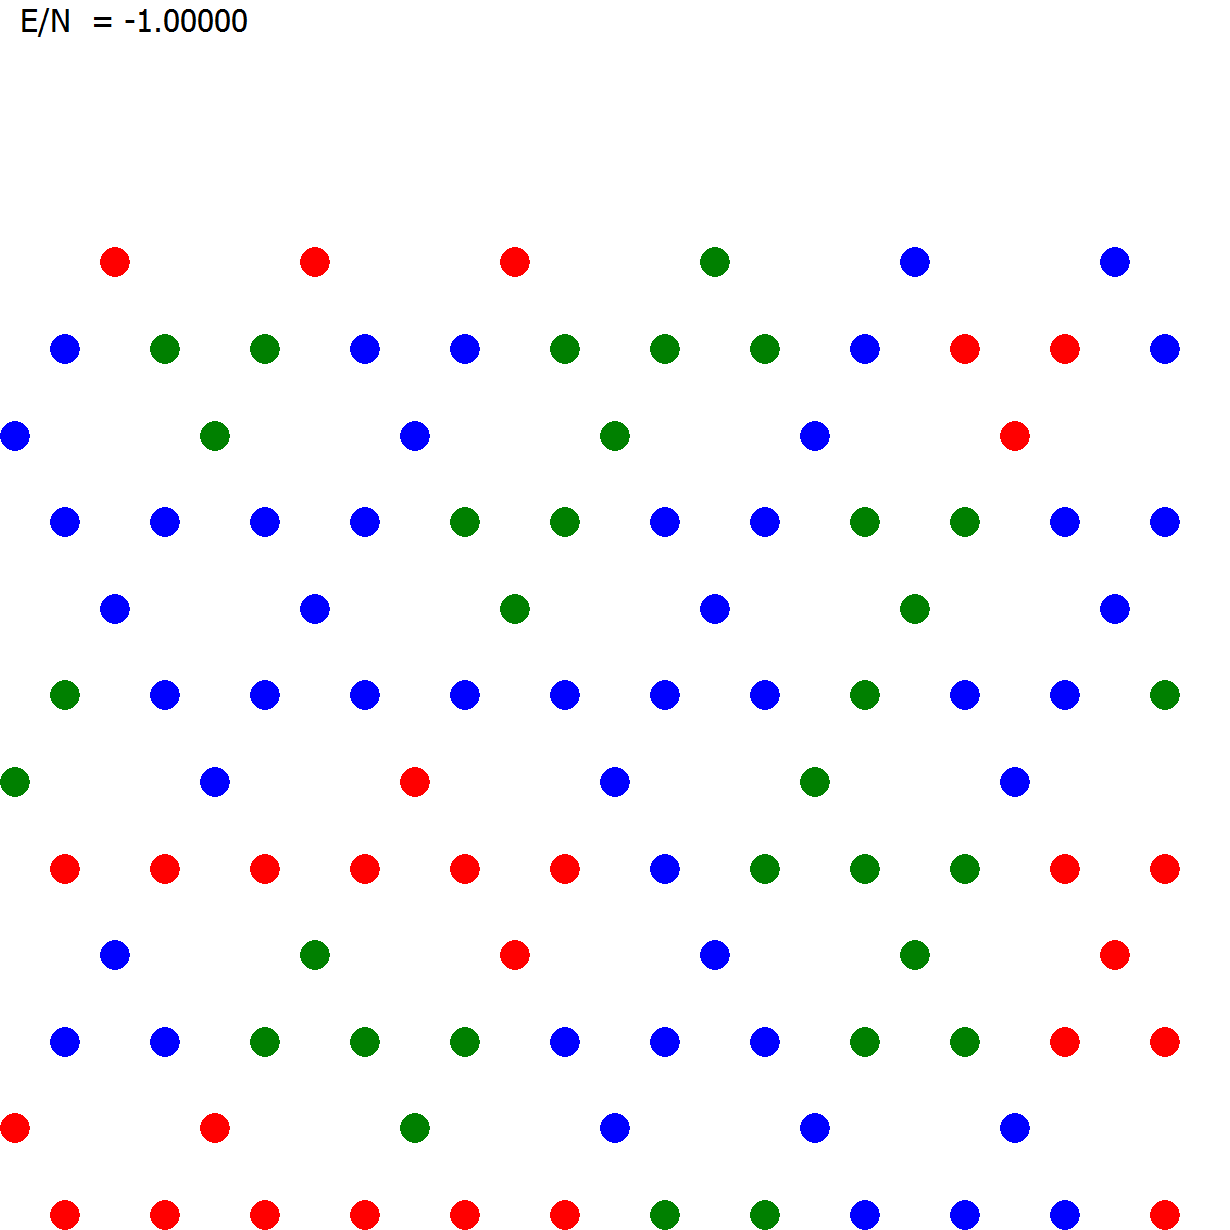
\includegraphics[width=1.0\textwidth]{mma/image25.png}
            \end{center}
            \caption{$J_2 = -0.5$.}
            \label{mma-fig-5}
        \end{subfigure}
        \begin{subfigure}{0.3\textwidth}
            \begin{center}
                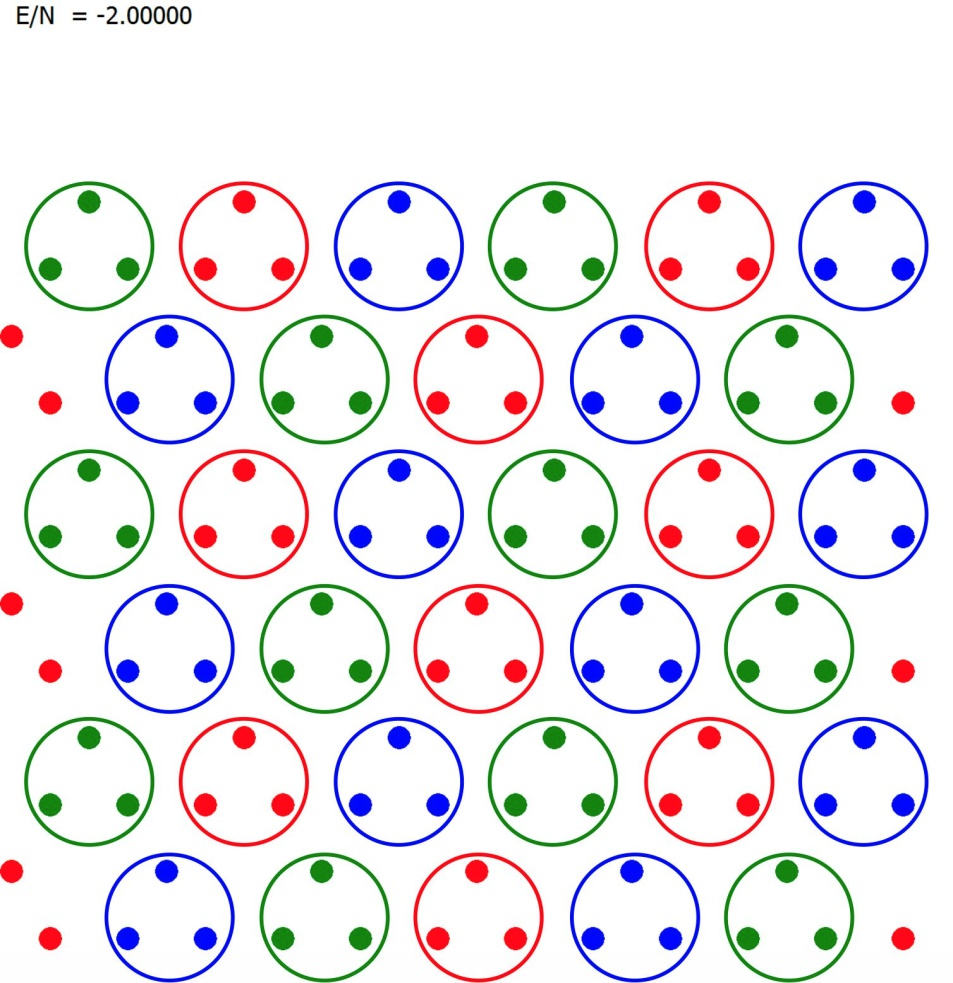
\includegraphics[width=1.0\textwidth]{mma/image26.jpeg}
            \end{center}
            \caption{$J_2 < -0.5$.}
            \label{mma-fig-6}
        \end{subfigure}
    \end{center}
    \caption{Структура основного состояния при разных значениях $J_2$.}
\end{figure}

Энергия основного состояния для ферромагнитной области задается как:
\begin{equation}
    \label{mma-eq-2}
    E_{\min} = -2J_1 - 2J_2.
\end{equation}

Энергия основного состояния для триплетной антиферромагнитной области задается как:
\begin{equation}
    \label{mma-eq-3}
    E_{\min} = - \frac{1}{2} J_1 + J_2.
\end{equation}

Вычислив единожды плотность состояний системы $g(E)$ можно легко рассчитать температурную зависимость любой интересующей нас величины. Например, внутренняя энергия $E$, свободная энергия $F$, и энтропия $S$ системы могут быть рассчитаны следующим образом \cite{mma-bib-14}:
\begin{gather}
    \label{mma-eq-4}
    E(T) = \frac{\sum_{E} Eg(E) e^{-E/k_B T}}{\sum_{E} g(E) e^{-E/k_B T}},
    \\
    \label{mma-eq-5}
    F(T) = -k_B T \ln \left( \sum_E g(E) e^{-E/k_B T} \right),
    \\
    \label{mma-eq-6}
    S(T) = \frac{E(T) - F(T)}{T},
    \\
    \label{mma-eq-7}
    C(T) = \frac{\langle E^2 \rangle - \langle E \rangle^2}{k_B T^2}.
\end{gather}

Рассчитанные из плотности состояний $g(E)$ по формулам \eqref{mma-eq-4}, \eqref{mma-eq-5}, \eqref{mma-eq-6}, \eqref{mma-eq-7} температурные зависимости внутренней энергии E и теплоемкости C при различных значениях обменных взаимодействий $J_1$ и $J_2$, для систем с линейными размерами $L=12$ и $L=36$ приведены на рисунках \ref{mma-fig-7} и \ref{mma-fig-8} соответственно. Отметим важную особенность алгоритма Ванга-Ландау: значения любых термодинамических параметров можно определить для любой температуры, с любым шагом, при этом объем необходимых вычислений, в отличие от других классических алгоритмов метода Монте-Карло, вырастает незначительно.
\begin{figure}[h]
    \begin{center}
        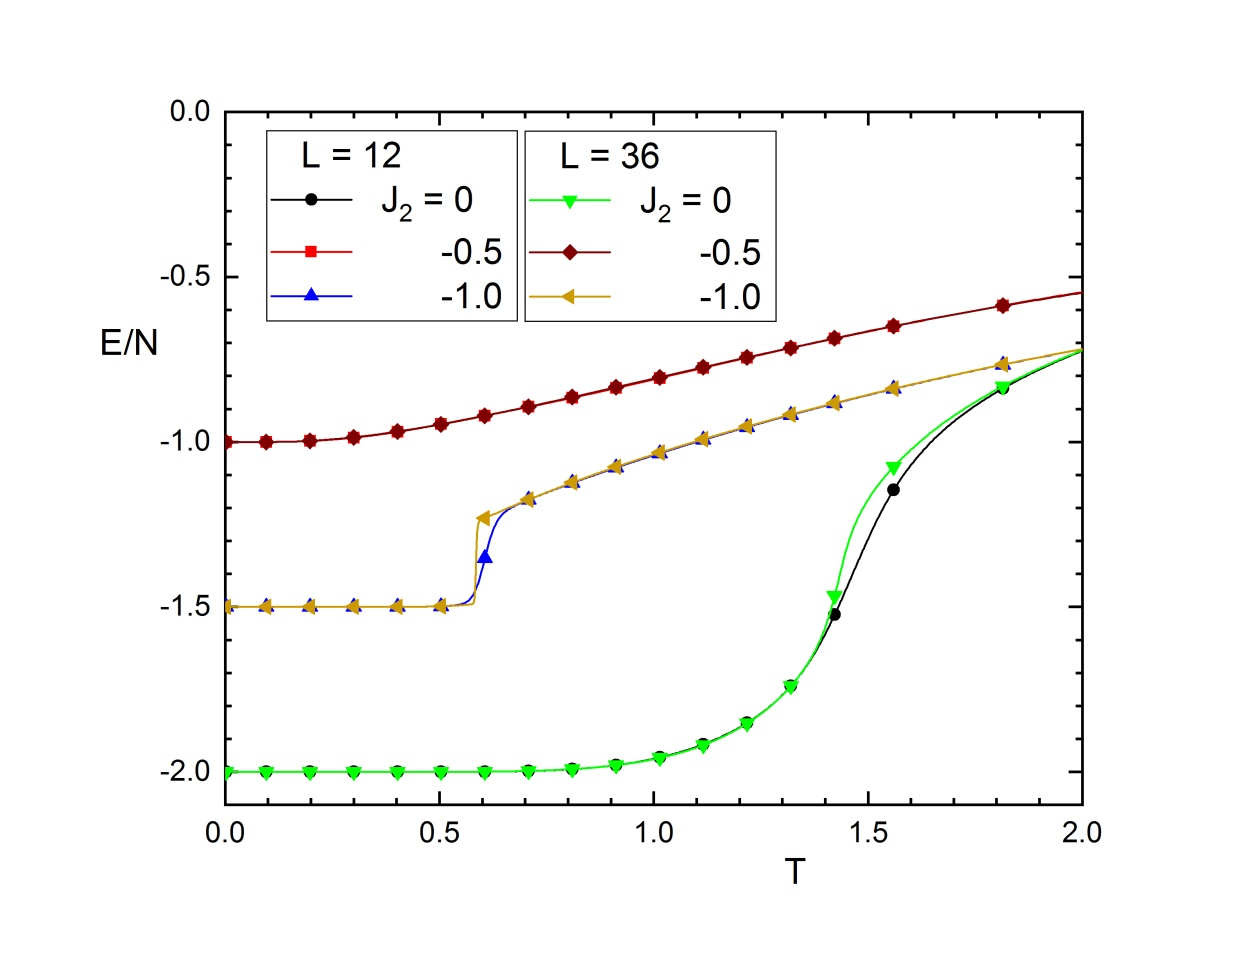
\includegraphics[width=0.5\textwidth]{mma/image31.jpeg}
    \end{center}
    \caption{Температурные зависимости внутренней энергии $E$, рассчитанные из плотности состояний $g(E)$ при различных значениях $J_1$ и $J_2$.}
    \label{mma-fig-7}
\end{figure}
\begin{figure}[h]
    \begin{center}
        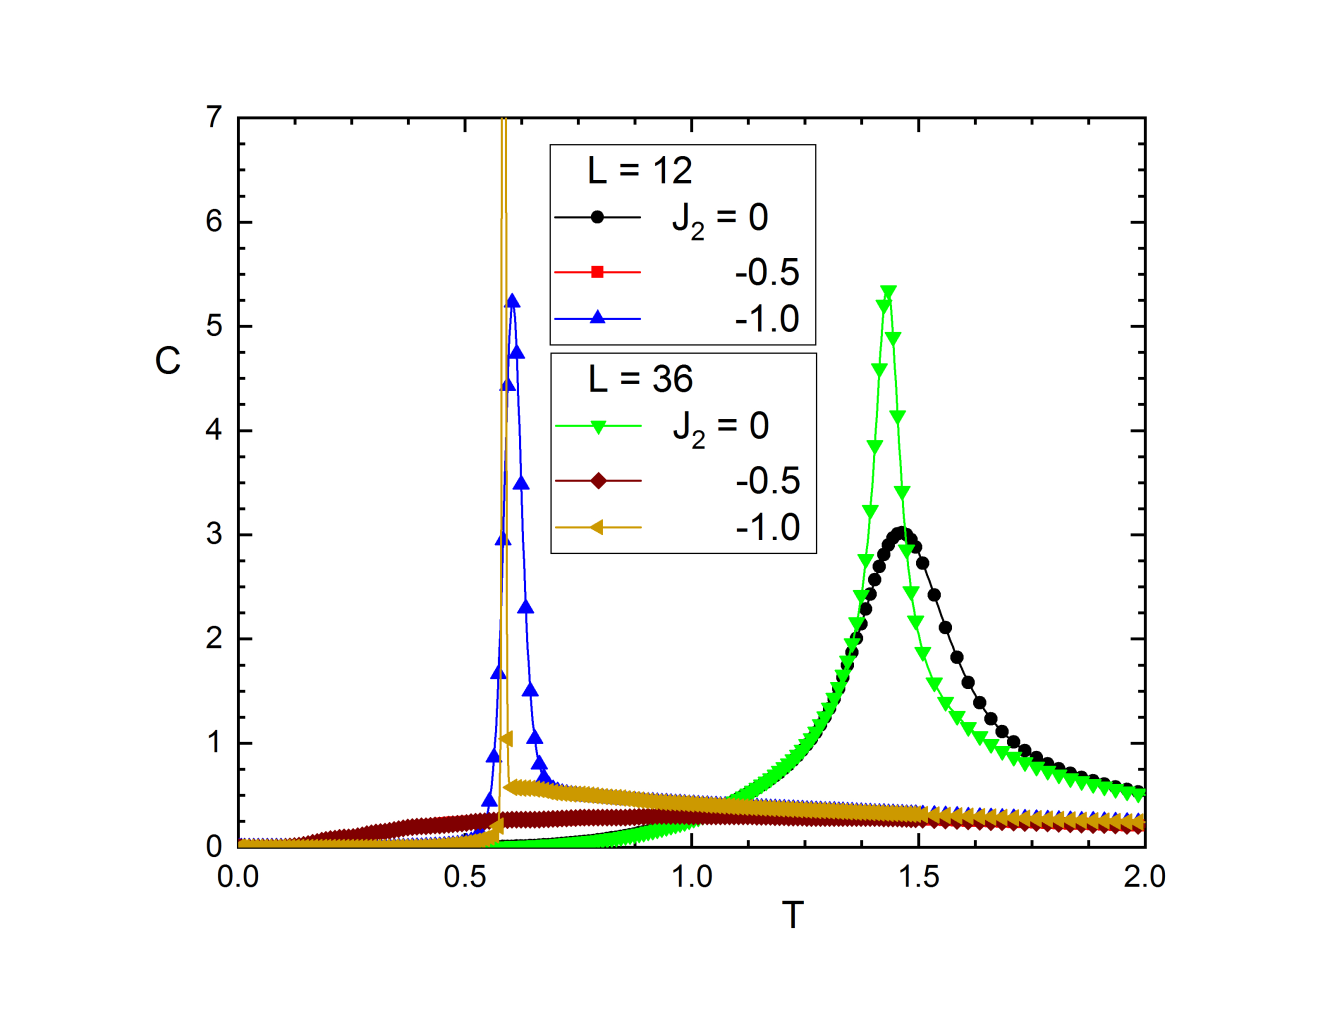
\includegraphics[width=0.5\textwidth]{mma/image32.png}
    \end{center}
    \caption{Температурные зависимости теплоемкости $C$, рассчитанные из плотности состояний $g(E)$ при различных значениях $J_1$ и $J_2$.}
    \label{mma-fig-8}
\end{figure}

Из рисунка \ref{mma-fig-7} видно, что в случае в случае $J_2=-1$ на графике наблюдается энергетический скачок, что говорит о фазовом переходе первого рода. Температурная зависимость теплоемкости, приведенная на рисунке \ref{mma-fig-8}, подтверждает эти предположения. В случае $J_2=-0.5$ скачка теплоемкости не наблюдается, в системе в данном случае не происходит фазового перехода. При $J_2=0$ происходит фазовый переход второго рода.

Для более подробного анализа фазовых переходов и определения типа перехода мы использовали гистограммный метод анализа данных.

Если рассчитать гистограмму по энергии по формуле:
\begin{equation}
    \label{mma-eq-8}
    P(E) = g(E) e^{-E/k_B T}
\end{equation}
то в области фазового перехода мы будем наблюдать два пика для фазового перехода первого рода и один максимум для фазового перехода второго рода.

На рисунке \ref{mma-fig-9} приведены гистограммы энергий в области фазового перхода при $J_2 = -1$ и $J_2 = 0$. Как видно из рисунка при $J_2 = -1$ в системе происходит фазовый переход первого рода, а при $J_2 = 0$ фазовый переход второго рода.
\begin{figure}[h]
    \begin{center}
        \begin{subfigure}{0.45\textwidth}
            \begin{center}
                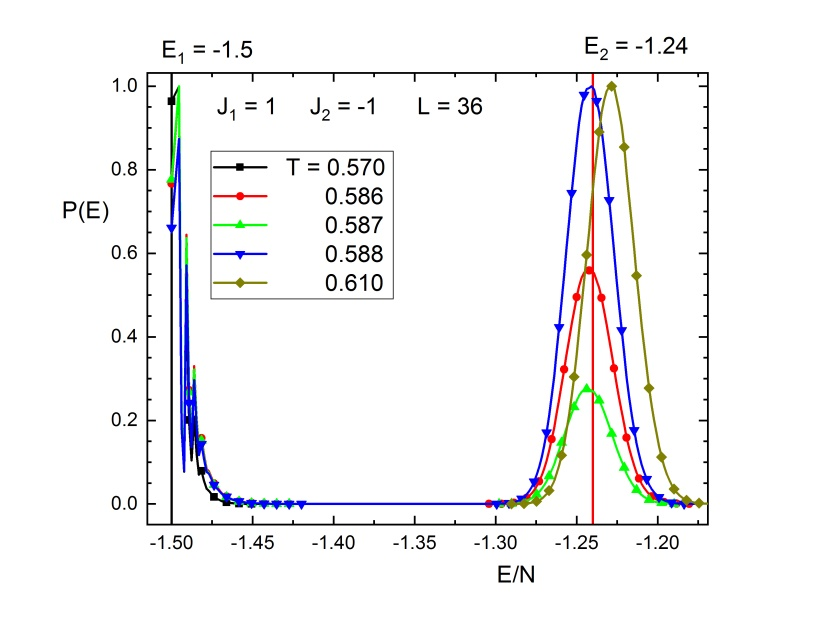
\includegraphics[width=1.0\textwidth]{mma/image34.jpeg}
            \end{center}
        \end{subfigure}
        \begin{subfigure}{0.45\textwidth}
            \begin{center}
                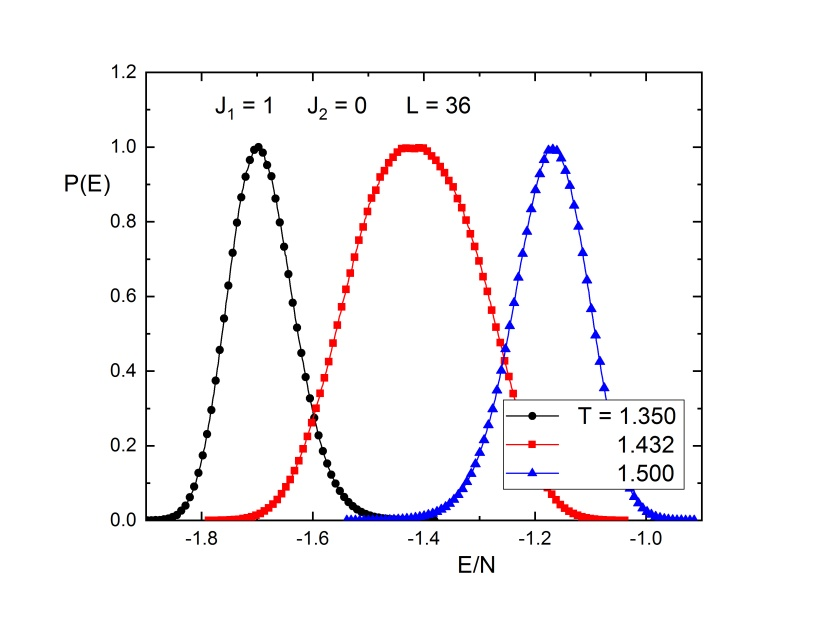
\includegraphics[width=1.0\textwidth]{mma/image35.jpeg}
            \end{center}
        \end{subfigure}
    \end{center}
    \caption{Температурные зависимости энтропии $S$, рассчитанные из плотности состояний $g(E)$ при различных значениях $J_1$ и $J_2$.}
    \label{mma-fig-9}
\end{figure}

Температурные зависимости энтропии $S$ при различных значениях обменных взаимодействий $J_1$ и $J_2$ для систем с линейными размерами $L=12$ и $L=36$ приведены на рисунке \ref{mma-fig-10}. При $J_2 = -0.5$ с понижением температуры энтропия стремится к значению $S_0/N = 0.435$, что говорит о сильном вырождении основного состояния. В остальных случаях с понижением температуры энтропия стремится к нулю. С повышением температуры для всех систем энтропия стремится к значению $\ln3 = 1.09861$.
\begin{figure}[h]
    \begin{center}
        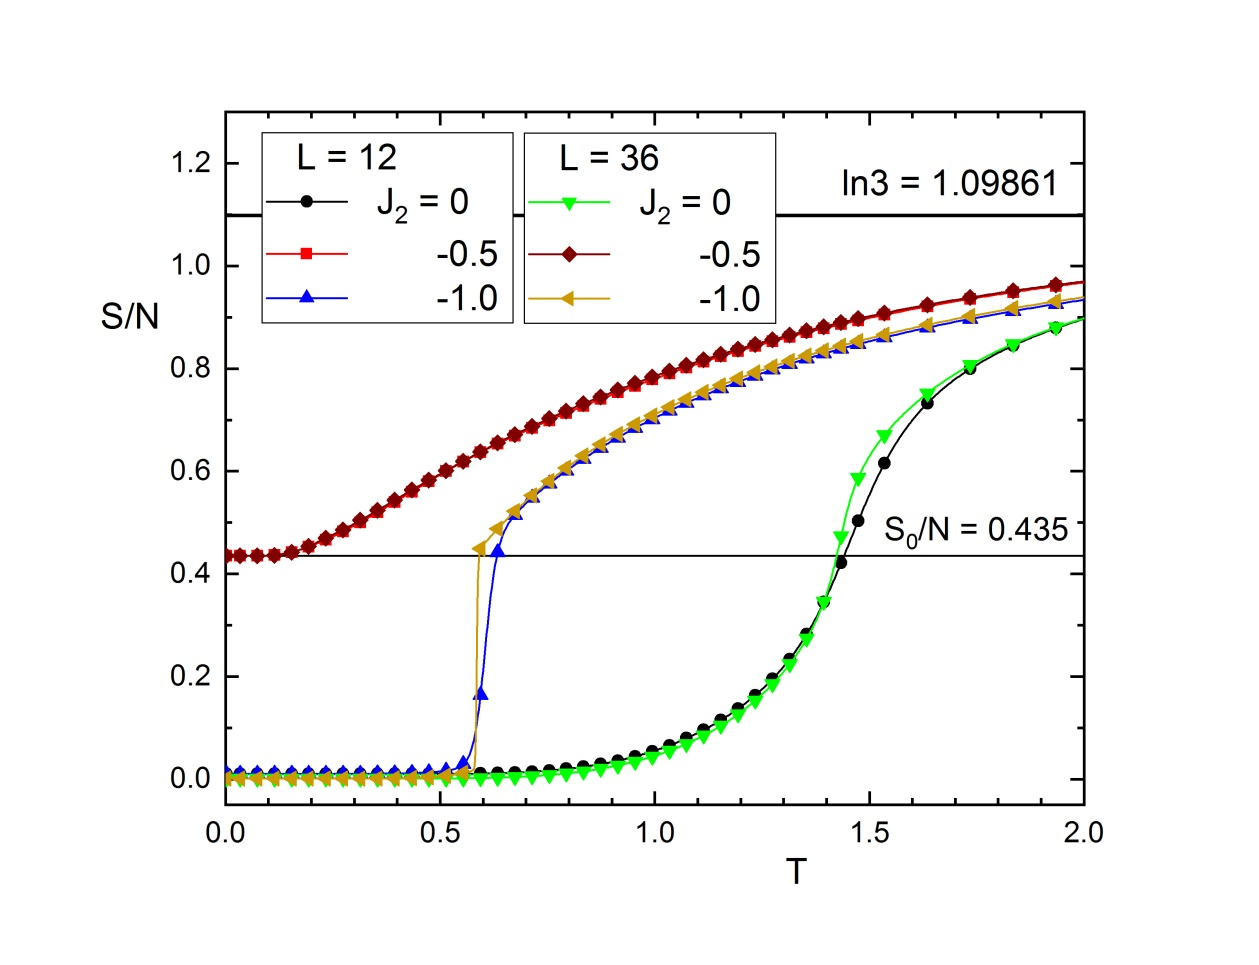
\includegraphics[width=0.5\textwidth]{mma/image36.jpeg}
    \end{center}
    \caption{Температурные зависимости энтропии $S$, рассчитанные из плотности состояний $g(E)$ при различных значениях $J_1$ и $J_2$.}
    \label{mma-fig-10}
\end{figure}

Анализ приведенных выше результатов позволило построить фазовую диаграмму, которая приведена на рисунке \ref{mma-fig-11}.
\begin{figure}[h]
    \begin{center}
        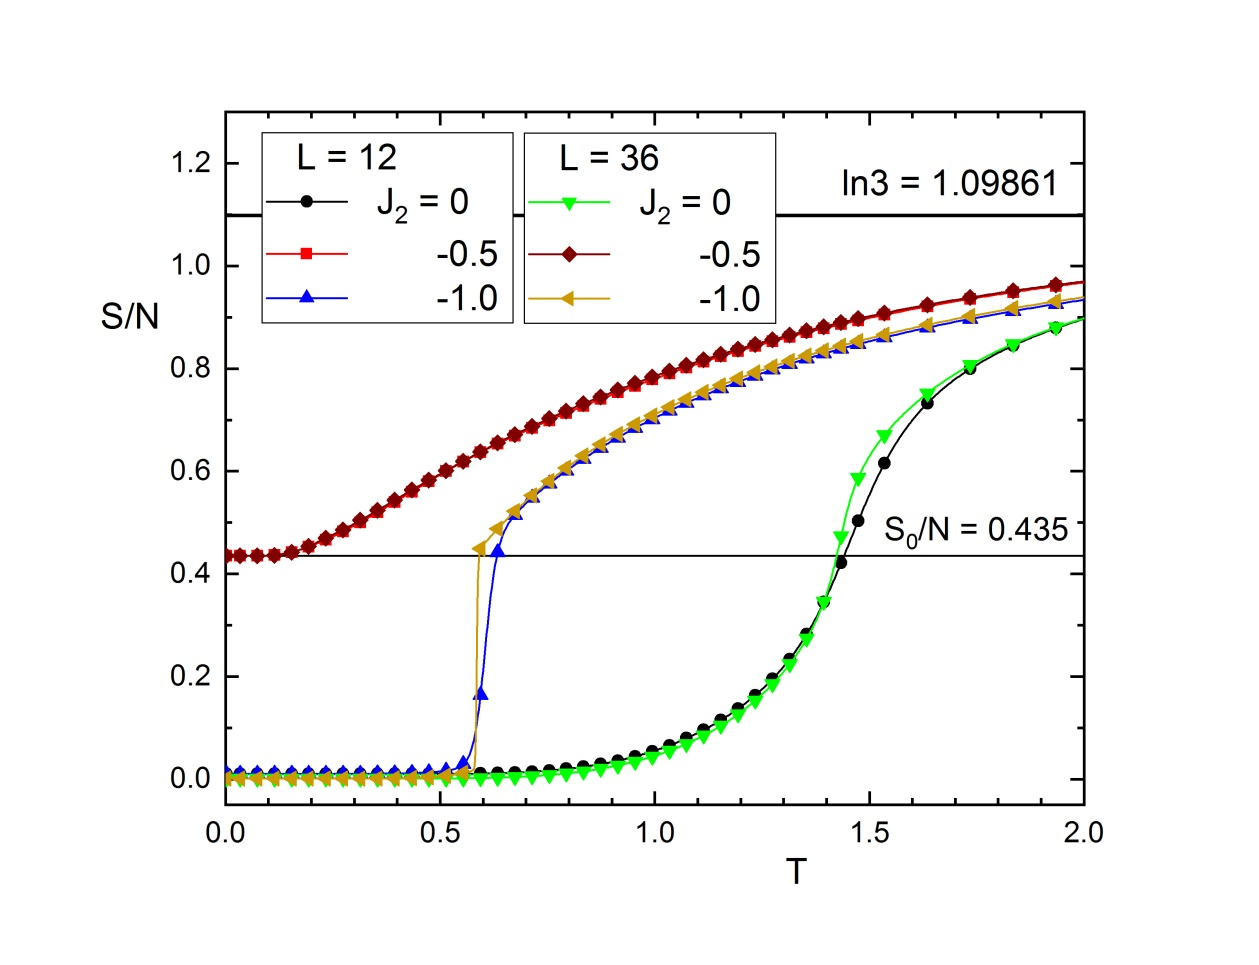
\includegraphics[width=0.5\textwidth]{mma/image36.jpeg}
    \end{center}
    \caption{Фазовая диаграмма.}
    \label{mma-fig-11}
\end{figure}


\section*{Заключение}

Исследование магнитных структур основного состояния, фазовых переходов и термодинамических свойств двумерной модели Поттса с числом состояний спина $q=3$ на решетке Кагоме с учетом взаимодействий первых и вторых ближайших соседей выполнено с использованием алгоритма Ванга-Ландау метода Монте-Карло. Получены магнитные структуры основного состояния в широком интервале значений величины взаимодействия вторых ближайших соседей. Построена фазовая диаграмма зависимости критической температуры от величины взаимодействия вторых ближайших соседей. Для значения $\left| J_2/J_1 = 0.5 \right|$ наблюдается вырождение основного состояния, и система становится фрустрированной.

Таким образом, по проделанной работе можно сделать следующие выводы:
\begin{itemize}
    \item Предложена модель Поттса с числом состояний $q=3$ на решетке Кагоме, учитывающая обменное взаимодействие между первыми и вторыми ближайшими соседями;
    \item Разработана программа для ЭВМ, основанная на новейшем алгоритме Ванга-Ландау, позволяющая исследовать модель Поттса с числом состояний $q=3$ на решетке Кагоме;
    \item Методом Ванга-Ландау вычислены плотности состояний $g(E)$ для модели Поттса с числом состояний $q=3$ на решетке Кагоме.
    \item Определены магнитные структуры основного состояния при различных значениях обменных взаимодействий и показано, что основное состояние может быть ферромагнитным (при $J_2 > -0.5$), триплетным антиферромагнитным (при $J_2 < -0.5$) или сильно вырожденным неупорядоченным фрустрированным (при $J_2 = -0.5$);
    \item Рассчитаны температурные зависимости различных термодинамических параметров, таких как свободная энергия $F$, внутренняя энергия $E$, энтропия $S$, теплоемкость $C$;
    \item Показано, что энтропия для данной модели при температурах близких к абсолютному нулю, при различных соотношениях обменных взаимодействий близка к нулю, кроме случая $J_2 = -0.5$, которое соответствует сильно вырожденному фрустрированному состоянию. С повышением температуры энтропия во всех случаях стремится к теоретически предсказанному значению $\ln 3$;
    \item Вычислены температуры фазовых переходов и определены типы фазовых переходов, происходящих в системе при различных значениях обменных взаимодействий. Построена фазовая диаграмма модели.
\end{itemize}

Результаты, полученные в ходе исследований, могут быть полезными для описания различных низкоразмерных магнитных материалов, имеющих структуру типа решетки Кагоме, таких как Гербертсметиты, Делафосситы, Капелласиты, Фольбортиты и т.д.
